\chapter{Два отрывистых}
%\corner{64}
\vepsianrose

C утра они поднялись относительно неплохо, хоть сон и был почти что прерывистый\mdash то и дело кто\sdash нибудь, пошатываясь в ночи, брёл в уборную\mdash пенное требовало расплаты. Позавтракали печеньками, припасённой колбасой и сыром, потом залили чаю в термосы\mdash горячая еда будет у них только вечером, поскольку по~многолетней то~ли традиции, то ли привычке на обед они в~походе не~варили горячего.

\diagdash Что, тяжко?\mdash подтрунивал Адмирал, расхаживая по комнате.

\diagdash Шурик, отстань. Щас раскачаемся$\ldots$\mdash отвечала команда, потягивая чаёк.

Снаряжение, перепакованное вчера, они покидали в~машины уже как\sdash нибудь, не особо распихивая\mdash всё равно скоро перекладывать в другое авто, которое закинет их на стапель. Собравшись, Адмирал созвонился с~Олегом, классным мужиком в Гирвасе, который уже более тридцати лет занимается заброской туристов на сплавы\mdash у~него двор большой, хозяйство, козлятки бегают, куры, во дворе поленница красиво сложенная, коптилка для сала и~мяса. Одним словом\mdash класс! Дядька оказался что надо. Очутившись буквально через 10 минут в его дворе, они быстро всё с ним обговорили насчёт стоянки своих двух машин. Потом приобрели кусок копчёного сала и копчёный рулет\mdash Олег при них проверял свою замечательную коптилку и~подкидывал туда щепу.

Сплавщики под руководством Адмирала быстро переложили вещи и снаряжение в прицеп, а сами все влезли в видавший и лучшие годы 7\sdash местный джип. Свои авто Шурик с~Серёгой загнали во двор к Олегу и поплотнее припарковались, а Шурик ещё и по~привычке скинул клемму с аккумулятора на всякий случай. Вся эта подготовка заняла не более получаса.

И вот, наконец, старт! Олег повернул направо на старую дорогу Гирвас\thinspace\nobreakdash---\thinspace  Петрозаводск, которая была достаточно приличной. Далее, через километров 30, свернули направо на Нёлгомозеро, как было написано на указателе. Дорога практически сразу стала гравийной, впрочем, в~достаточно хорошем состоянии. Видно было по обочине, что её равняли грейдером совсем недавно, может даже в этом месяце.

Если до этого местность была с переменным успехом равнинной, то сейчас пошли холмы, спуски и подъёмы, крутые повороты между холмами. Пейзаж значительно стал меняться по мере приближения к Нёлгомозеру\mdash собственно озеру и одноимённому населённому пункту на последней трети пути заброски от Гирваса. Гравийка по\sdash прежнему шла отлично укатанной.

%	\begin{wrapfigure}{l}{1.0\textwidth}
	\begin{figure}[h]
		\centering
		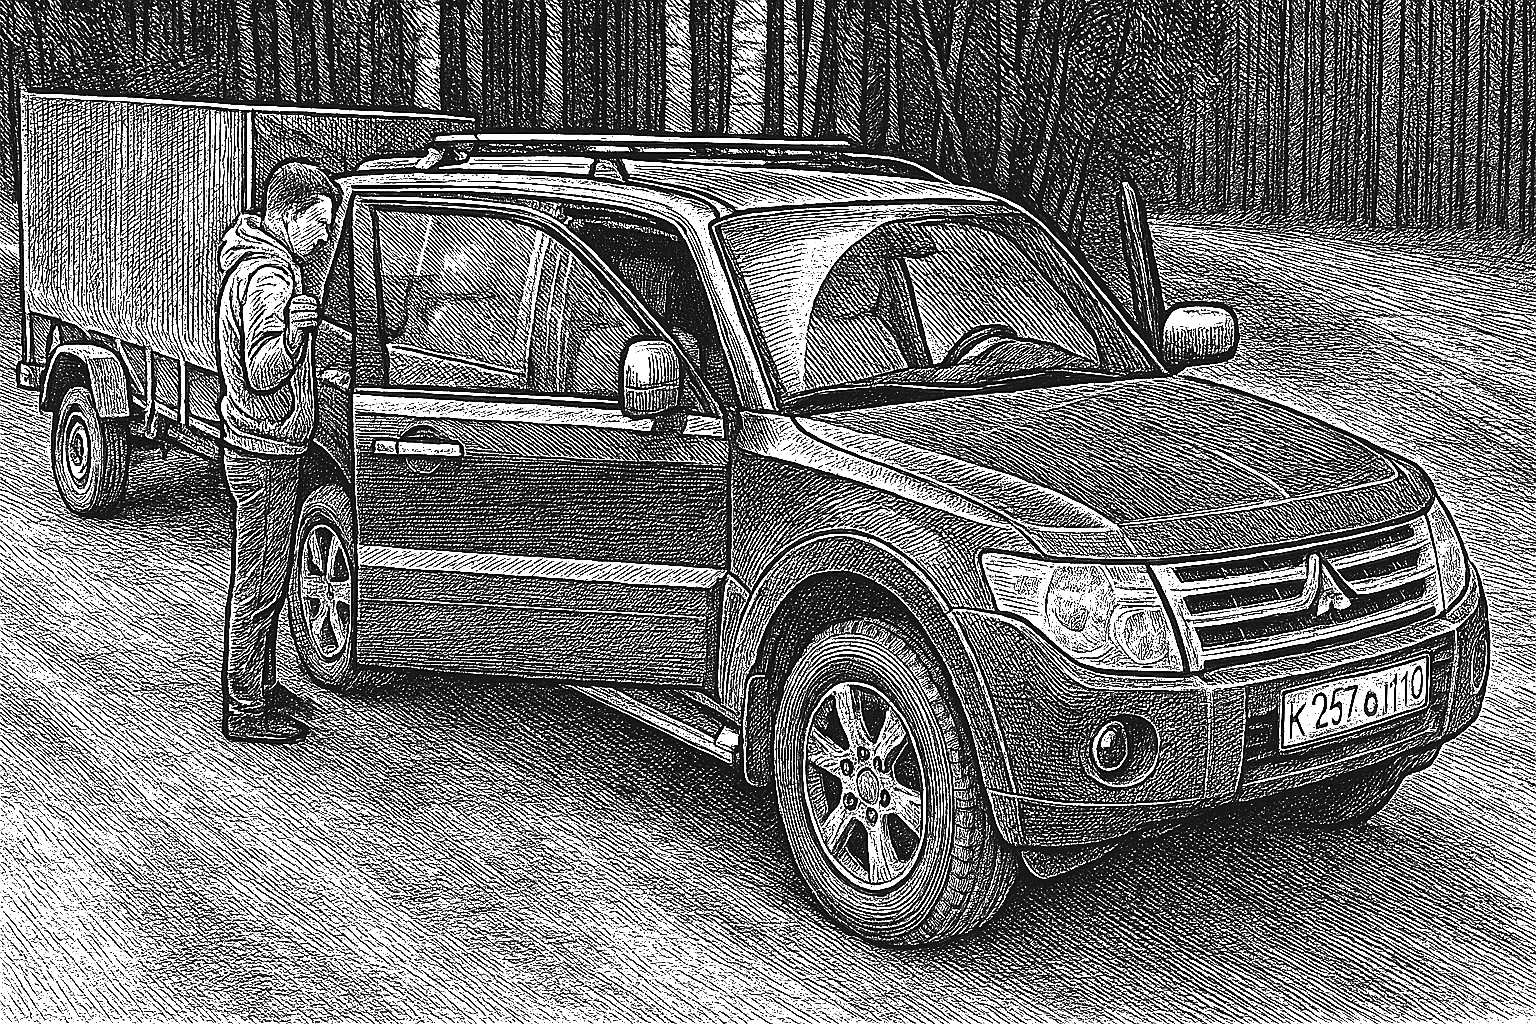
\includegraphics[width=1.0\textwidth]{10_1_jeep}
		\caption{\small\textit{...свернули направо на Нёлгомозеро...}}
	\end{figure}
%	\end{wrapfigure}

Адмирал, расположившись на переднем пассажирском рядом с Олегом, включил прибор GPS\footnote{GPS (англ. global positioning system) --- спутниковая система навигации.}. И вдруг его прошиб холодный пот:

\diagdash КИРЯ!!!\mdash чуть не заорал он.

\diagdash Что, утюг не выключил?\mdash участливо ответкой ввернул тот, встрепенувшись на третьем ряду сиденьев.

\diagdash Я забыл описание порогов$\ldots$

\diagdash !!!

\diagdash Едрёна мать! Карта есть, вся снаряга есть, всё есть, описание забыл на столе в Москве!!!\mdash Адмиралу даже сделалось дурно\mdash забыть можно было всё, что угодно, но~только не описание порогов. 

\diagdash Связь я даже не знаю, будет ли ещё$\ldots$\mdash глухо сказал Олег.

В посёлке Нёлгомозеро, к которому они подъехали, все стали неистово проверять свои мобильники. Только у~Кири появился Интернет, и даже удалось немного загрузить описание маршрута, спасая положение Адмирала:

\diagdash Так, Шурик, на половину маршрута прогрузилось!

\diagdash Уф\sdash ф\sdash ф!!!\mdash выдохнул Адмирал. Как он мог забыть описание? Воистину никогда не знаешь, что забудешь взять с собой. В контрольном листе лоция отчего\sdash то не значилась, вот он в~утренней запаре сборов тогда, два дня назад, и~не взял эту маленькую книжечку, оставив её на кухне у~телевизора\mdash как в~немом кино встала сейчас эта картина перед его глазами$\ldots$

%\newpage
\vspace{0.5cm}
$\ldots$Cплавщики наконец подъехали к крутому левому повороту, где направо вниз с~холма уходила грунтовка. 

\diagdash Приехали! Отсюда ближе всего до~воды.\mdash сказал Олег. Место согласовывалось с~адмиральской картой. 

\diagdash Окей! Команда, десантируемся!\mdash скомандовал Адмирал спешившись, и они стали спускаться по~ответвлению с дороги вниз. Гравийка, по которой они ехали сюда, шла по довольно высокой возвышенности водораздела между озёрами. Высота над уровнем воды была около пятнадцати метров, прикинул Адмирал, тяжко ступая кедами с холма. Сейчас они все шли вниз под нехилым уклоном, стремясь не грохнуться ненароком.

Олег, подумав, как лучше сделать, решил проехать вниз, врубив пониженную передачу в джипе\mdash зверь\nobreakdash\sdash\nobreakdash машина! Он~смог заехать на грунтовку в лес с~прицепом и~развернуться на хорошей большой поляне, которая, судя по~антикультурным следам цивилизации, часто использовалась под стапель. Площадка, что интересно, была почти ровной, но до и после неё уклоны уже шли приличные.

Водитель ювелирно развернулся в ограниченном пространстве с прицепом, подав последний задом к спуску вниз так, чтобы было удобно выкидывать тюки со снарягой ближе к озеру. Все манёвры он выполнял просто мастерски лавируя прицепом между валунами, торчащими из~склона. Наконец, всё было готово:

\diagdash Ну вот и всё, мужики! Разгружай!\mdash сказал Олег, закурив и открыв борт прицепа.

\diagdash Айда, пацаны! Разгружаемся!\mdash скомандовал Адмирал, и команда молниеносно перекидала весь свой скарб на черничник, буквально устилавший всё по краям лесной дороги, ниточкой украдкой пролегавшей по светлому сосновому лесу без подлеска. 

Сквозь деревья внизу виднелось сереющее озеро. Пока остальная часть команды доканчивала разгрузку, Адмирал, нацепив брезентовую штормовку и бежевую панаму, спустился вниз к~воде оценить место стапеля. 

\diagdash Терпимо$\ldots$\mdash сказал он сам себе задумчиво.\mdash Но~подъём просто трындец$\ldots$\mdash у воды ровной площадки не~было. Оставалось лишь собирать байдарки там, наверху, где выгрузились. Он пошёл обратно к команде.

Олег, тем временем, закрывал опустевший прицеп:

\diagdash Ну, мужики, удачи! Хорошего отдыха и рыбалки!\mdash пожелал он им и, обратясь к Адмиралу, продолжил,\mdash В~конце пути, когда озёра пойдут, и там связь уже будет, вы мне, короче, наберите за сутки, чтобы я знал? Вас забирать наверно не надо\mdash пешком до машин дойдёте?

\diagdash Ага, спасибо! Так и есть!\mdash поблагодарил Адмирал и расплатился за заброску.

Олег уехал, ещё раз пожелав им удачи. Команда сидела на вещмешках среди черничника, приходя в себя. Черничник уходил ещё выше вверх по склону, градусов под сорок, не~меньше. Рельеф был почти что горный в~понимании команды, привыкшей к равнинным пейзажам Чагодощенского края, где они сплавлялись в последние годы. Народ потихоньку приходил в себя, попивая чаёк из термосов. Адмирал ощутил немереный эмоциональный подъём\mdash скоро, они скоро будут на воде! Скоро они встанут на~воду, обводы байдарок рассекут водную гладь, и~вчерашние пешеходы преобразятся в~мореманов$\ldots$ 

%Надо было собирать плавсредства: 

%\renewcommand*{\thefootnote}{\fnsymbol{footnote}}
\renewcommand*{\thefootnote}{\arabic{footnote}}
\setcounter{footnote}{0}
\diagdash Так! А ну! Паша, Руслан! Ком цу мир\footnote{Подойдите ко мне (нем. komm zu mir).}! По цепочке становись! Принимай штевни\footnote{Штевни\mdash части корпуса, которыми заканчивается набор судна в~носу (форштевень) и~корме (ахтерштевень).}, черти!\mdash насел Адмирал на~свой экипаж, открыв упаковку с байдаркой.

\diagdash Серёга! Погнали!\mdash Замполит тоже привлёк своего матроса к сборке их байды\sdash двушки.\mdash Ща мы их сделаем!

\diagdash Хрена два!\mdash распалялся Адмирал.\mdash Лом вам абордажный во все дыры!!! 

%\renewcommand*{\thefootnote}{\fnsymbol{footnote}}
\renewcommand*{\thefootnote}{\arabic{footnote}}
\setcounter{footnote}{0}
\diagdash Шурик, хар\'{о}ш! Чё дальше собирать?\mdash Паша уже закрепил носовой и кормовой штевни в пазы кильсонов\footnote{Кильсон (англ. keelson)\mdash продольная составная часть одинарного дна корпуса речного судна (\textit{здесь и далее морские термины приводятся по}\cite{МорскойСправочник}).}, которые Адмирал состыковал и разложил внутри расправленной на траве байдарочной шкуры.

\diagdash Да, ты командуй как что.\mdash отозвался Руслан, пытаясь понять принцип сборки байдарки.

Адмирал привычными движениями осуществлял священнодейство\mdash превращал вместе со своим экипажем гору дюралевых трубок и ПВХ\sdash шную\footnote{Поливинилхлорид\mdash материал, пришедший на смену брезенту при изготовлении оболочек (<<шкур>>) байдарок <<Таймень>> и другого туристического снаряжения.} шкуру в огромную трёхместную байдарку <<Таймень>>. Вынимая очередной шпангоут\footnote{Шпангоут (гол. spanthout, spant\mdash ребро, hout\mdash дерево)\mdash криволинейная поперечная балка корпуса судна, подкрепляющая наружную обшивку и обеспечивающая прочность и устойчивость бортов и днища.} из упаковки, он вдруг завис, держа в~одной руке откуда\sdash то взявшийся кормовой кильсон от~байды\sdash двушки и~почесывая другой рукой затылок:

\diagdash Ё-ё-ё!

%\renewcommand*{\thefootnote}{\fnsymbol{footnote}}
%\renewcommand*{\thefootnote}{\arabic{footnote}}
%\setcounter{footnote}{0}
\diagdash Чё, Шурик, кильсон не тот\footnote{Кормовые кильсоны байдарок <<Таймень-2>> и <<Таймень-3>> отличаются, не взаимозаменяемы.} взял?\mdash мигом нарисовался Замполит.

\diagdash Ты не поверишь, лишний взял!!!

\diagdash Гы-гы-гы!!!\mdash загоготала команда.

\diagdash Адмирал, ты не говорил, что пороги такие, что надо брать запасной каркас!\mdash Замполит веселился, ставя шпангоуты.

\diagdash Смейся, смейся! Ща как тридцаточку под дождём попрёмся!\mdash глухо отозвался Адмирал.\mdash В прошлый\sdash то раз на двушке ходили, вот я и взял упаковку целиком, особо не~проверяя, закинул только кильсон на трёшку, а~двушечный как лежал в упаковке, так и остался. Ну, Кирь, тебе запасной будет, если чё!\mdash подытожил он наконец.

\diagdash Не-не-не, не надо никаких <<если чё>>!\mdash парировал Серёга, собирающий их с Кирей двушку.

%\renewcommand*{\thefootnote}{\fnsymbol{footnote}}
\renewcommand*{\thefootnote}{\arabic{footnote}}
\setcounter{footnote}{0}
\diagdash Так, теперь самое сложное\mdash натяжка бортов, парни! Тащ м\'{о}трос, давай помогай!\mdash скомандовал Адмирал Руслану и, кряхтя, принялся защёлкивать замки фальшборта\footnote{Фальшборт (нем. Falschbord)\mdash пояс, расположенный выше верх. палубы судна, выполнен как продолжение борта.}. Это было непростой операцией.

\diagdash Слушай, Юрич как\sdash то легко это делал.\mdash глядя на~их~страдания, сказал Паша.

\diagdash Помогай! Он так и делал\mdash в живот борт упирал, массой тела давил сверху и защёлкивал эти хренюшки!\mdash отозвался, кряхтя, свесившись над последним замком левого борта, Адмирал. 

Замок наконец\sdash то защёлкнулся:

\diagdash Уф\sdash ф\sdash ф!

\diagdash Это был детский сад. Сейчас самая жесть\mdash второй борт.\mdash Адмирал присел передохнуть, он был уже весь в~мыле. Киря и Серёга ещё копошились со~стрингерами\footnote{Стрингер (от англ. string)\mdash продольный элемент набора корпуса судна.}: 

\diagdash У-у-у, тащ Замполит, чёта у вас таки халтура!

\diagdash Адмирал, за вами таки не угнаться!

{
%	\begin{wrapfigure}{l}{1.0\textwidth}
	\setlength{\belowcaptionskip}{-9mm}
\begin{figure}[h]
	\centering
	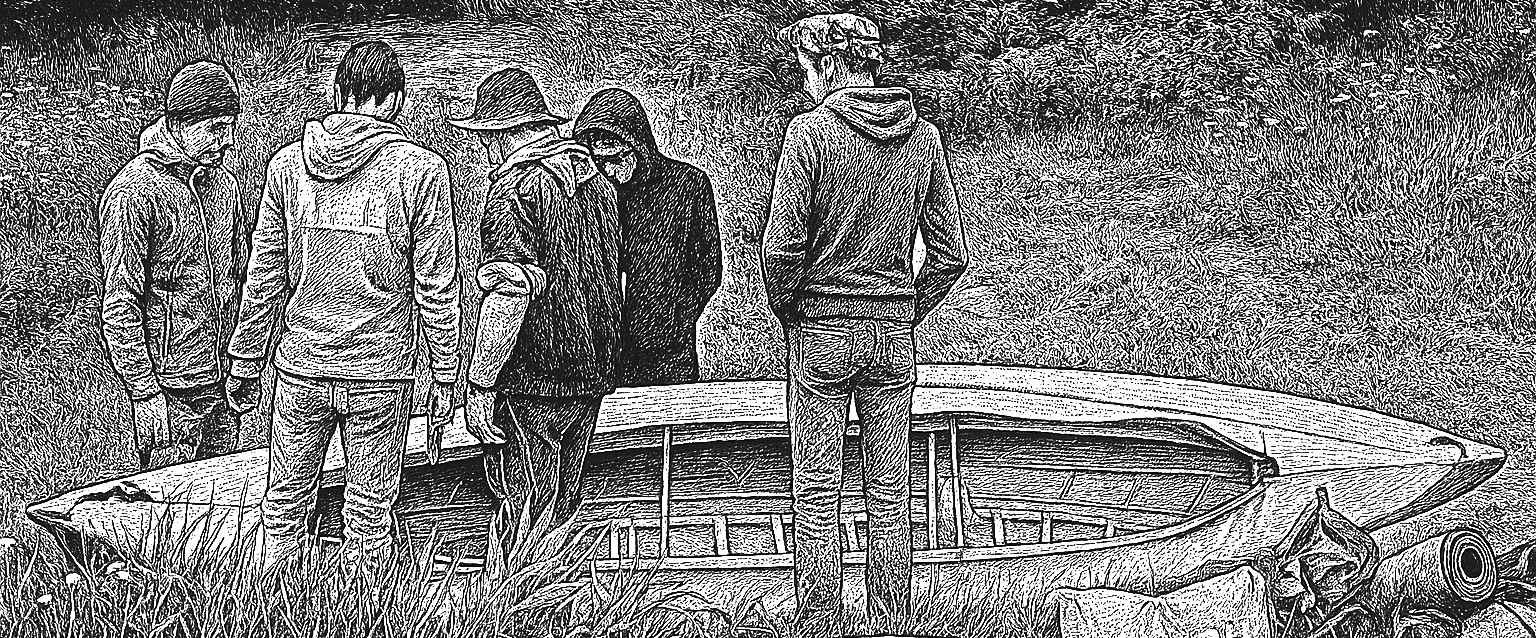
\includegraphics[width=1.0\textwidth]{11_1_keelson}
	\caption{\small\textit{...фальшборт не лезет...}}
\end{figure}
%	\end{wrapfigure}
}

\diagdash А то! Так, парни, второй борт. Паш, подсоби! Руслан, смотри чтоб шкура из паза не выходила, ставим на борт!\mdash они повернули байду на другой борт и стали натягивать оболочку, стремясь попасть замками в предназначенные для них отверстия. Это было непросто\mdash шкура была из ПВХ и~практически не тянулась, ребята умаялись.

\diagdash Не входит один, глянь!\mdash показал Паша Адмиралу.

\diagdash Ща! При помощи пассатижей и какой\sdash то матери, как обычно!\mdash хохотнув, молвил Адмирал и достал из вещмешка с байдарочными принадлежностями пассатижи\sdash кобру. Подогнув ими полукруглое ответное <<ухо>> замка, ребята снова налегли на фальшборт:

\diagdash Делай раз: жми что есть мочи!\mdash скомандовал Адмирал и они с Русланом упёрлись животами в борт,\mdash Делай два: закрывай!!!\mdash Паша застёгивал замки.

\diagdash Есть контакт, застегнули!\mdash они все втроём поставили наконец\sdash то собранную байду на ровный кильсон.\mdash Фу\sdash у\sdash у\sdash ух!!! Можно выдохнуть маленько. Замполит, смотри как профи работают!\mdash Адмирал был удовлетворён командной работой своего экипажа при сборке.

\diagdash Шурик, помогай, блин! Фальшборт не лезет!\mdash Киря пыхтел над байдой.

\diagdash Погоди, ща перекурим и сбацаем.\mdash Адмирал и Паша устало присели на мшаник и задымили. Киря и Серёга всё ещё возились. 

\diagdash Шурик!!!\mdash не унимался Киря.

\diagdash ИДУ!\mdash Адмирал тяжело поднялся, подошёл к~кириной байде,\mdash Так, чё тут?\mdash и, увидев, что тут та же самая картина с бортом, как была и на его ласточке пару минут назад, поставил байду на борт, благо двушка легче. 

Киря упёрся животом в борт, таща руками противоположный фальшборт на себя:

\diagdash Ещё!!!

\diagdash Уф-ф-ф!\mdash Адмиралу удалось застегнуть замок пассатижами.\mdash Ну вот! А то возитесь, возитесь, Ы!

\diagdash Вот те и Ы!\mdash Замполит смахнул пот со лба, умаявшись, и сел передохнуть.

Пашка перекурил, поправил свою широкополую шляпу и оживился:

%\diagdash А чё, давайте, может?$\ldots$\mdash хитрая ухмылочка не~оставляла сомнений в его намерениях, Адмирал сразу просёк тему.

\diagdash А чё, давайте, может$\quldots$\mdash хитрая ухмылочка не~оставляла сомнений в его намерениях, Адмирал сразу просёк тему.

\diagdash Ну по чуть-чуть можно, пожалуй$\ldots$\mdash неуверенно поддержал Замполит.

%\diagdash Ладно, черти! Погода портится, щас ливанёт. Сугубо в терапевтических целях!!!\mdash отозвался Адмирал и~пошёл к~вещмешкам нарушать неписаные законы трезвости на~воде, поборником которых он являлся. Но не сегодня\mdash Адмирал задолбался при сборке байд и подумал, что заряд \makebox[\linewidth][s]{\noindent ямайского рома никому не повредит. Даром что ли}

\diagdash Ладно, черти! Погода портится, щас ливанёт. Сугубо в терапевтических целях!!!\mdash отозвался Адмирал и~пошёл к~вещмешкам нарушать неписаные законы трезвости \makebox[\linewidth][s]{\noindent на~воде, поборником которых он являлся. Но не сегодня\mdash} 

%\begingroup
%\justifying
%\parfillskip=0pt % <- это заставит последнюю строку растягиваться
%
%в терапевтических целях!!!\mdash отозвался Адмирал и пошёл 
%
%\par
%\endgroup

%\newpage

{
%	\begin{wrapfigure}{l}{1.0\textwidth}
	\setlength{\belowcaptionskip}{-25pt}
	\begin{figure}[h]
		\centering
		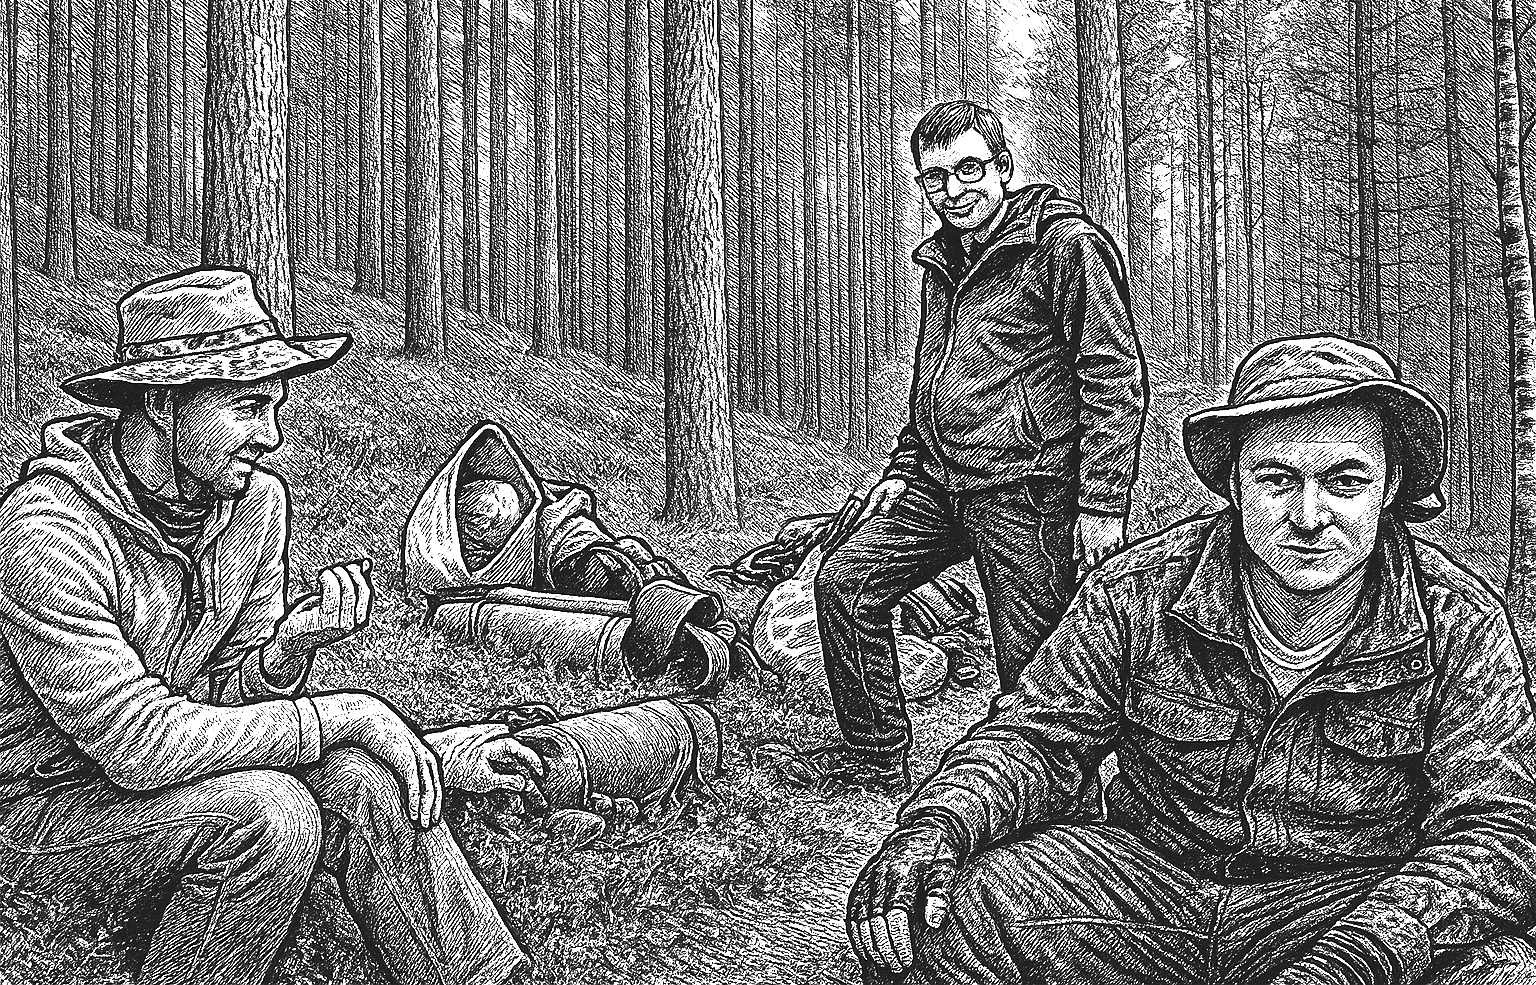
\includegraphics[width=1.0\textwidth]{12_2_maybe}
		\caption{\small\textit{...А чё, давайте, может?..}}
	\end{figure}
%	\end{wrapfigure}
}

\noindent Адмирал задолбался при сборке байд и подумал, что заряд ямайского рома никому не повредит. Даром что ли на британском флоте только в 1970\sdash м году отменили многолетнюю традицию раздачи рома морякам.  

%Адмирал задолбался при сборке байд и подумал, что заряд \makebox[\linewidth][s]{\noindent ямайского рома никому не повредит. Даром что ли}
%
%\noindent на британском флоте только в 1970\sdash м году отменили многолетнюю традицию раздачи рома морякам.  

\diagdash А ну, команда! Ком цу мир! Подставляй!\mdash железные кубки брякнули, живительная влага наполнила их.

\diagdash Тащ Адмирал, толкни речь!\mdash повелевал Замполит.


\begingroup
\justifying
\parfillskip=0pt % <- это заставит последнюю строку растягиваться


\diagdash Ессесно. Кхм!\mdash Адмирал докуривал сигарку,\mdash Итак! Начинается наш сплав <<Сунская цепочка>>! Стапель пройден\mdash байдарки собраны, вот они, пжалста!\mdash и~повёл рукой в их сторону.\mdash Щас мы чайком, тэк скэзэть, усугубим и пойдём по озеру$\ldots$ Как оно называется, Кирь?

\par
\endgroup

%\noindent Стапель пройден\mdash байдарки собраны, вот они, пжалста!\mdash и повёл рукой в их сторону.\mdash Щас мы чайком, тэк скэзэть, усугубим и пойдём по озеру$\ldots$ Как оно называется, Кирь?

\diagdash Вендюрское! 

%\diagdash Да, точно! По Вендюрскому озеру!
\makebox[\linewidth-\parindent][s]{\diagdash Да, точно! По Вендюрскому озеру! Сегодня нас}

\begin{wrapfigure}[10]{l}{0.52\textwidth}
\setlength{\belowcaptionskip}{-10pt}
%	\begin{figure}[h]
\centering
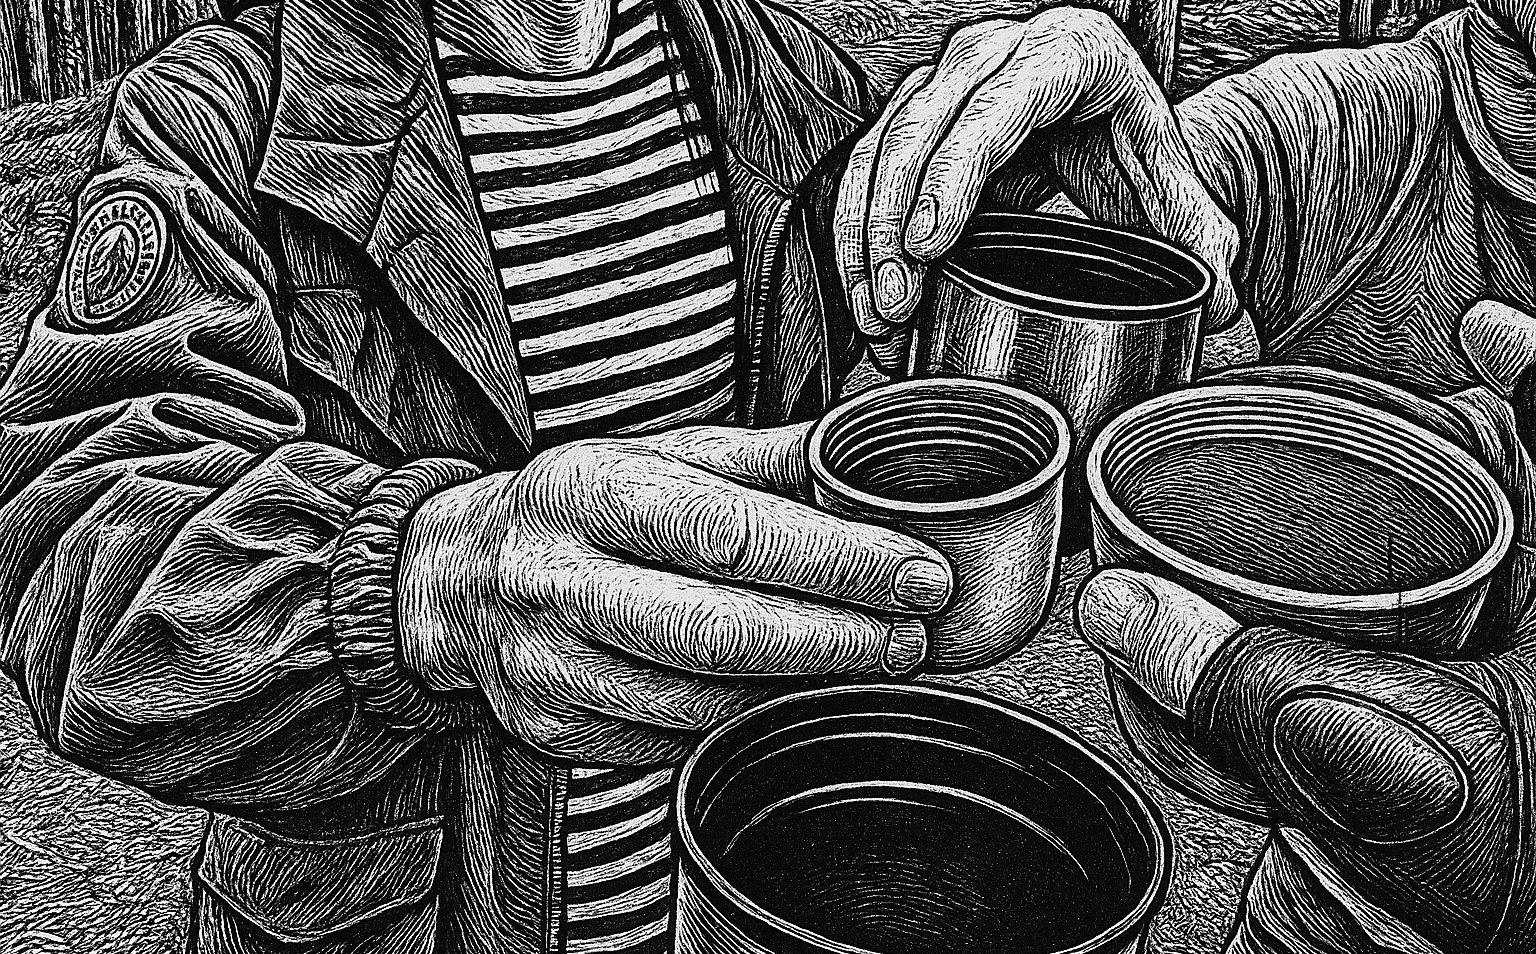
\includegraphics[width=0.52\textwidth]{13_skol}
\caption{\small\textit{...два отрывистых...}}
%	\end{figure}
\end{wrapfigure}

\noindent ждут каналы между озёрами ещё, кстати. Итак, то, к~чему мы стремились\mdash свершается! Мы выбрались в наш первый совместный сплав по Карелии и, надеюсь, это приключение запомнится нам надолго! Ну,~мужики, будем!\mdash лес рук с кружками поднялся и замер, ожидая команды.\mdash Тащ~Замполит, два отрывистых и одно раскатистое!!!

\diagdash {\large УРА, УРА, УРА\sdash А\sdash А!!!}\mdash грянуло над стапелем, эхом отражаясь в светлом сосновом бору.

%\newpage


	
%\noindent
%\begin{minipage}{0.57\textwidth}
%	\centering
%	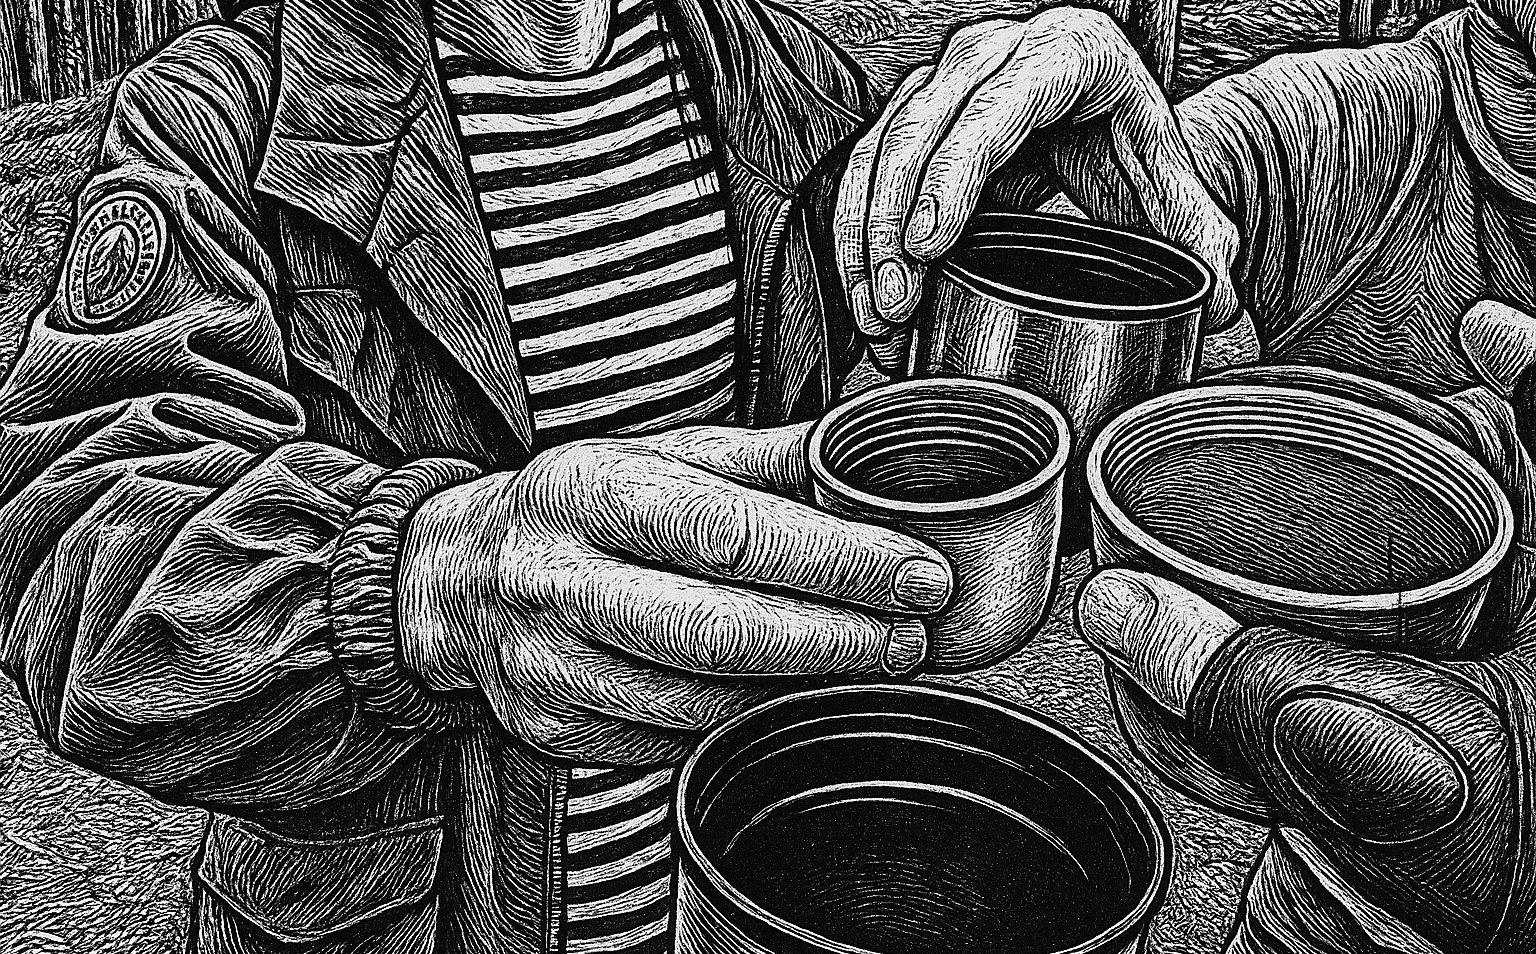
\includegraphics[width=0.999\linewidth]{chok3}
%	
%	{\small\textit{...два отрывистых и одно раскатистое!...}}
%\end{minipage}\hfill	
%\begin{minipage}{0.38\textwidth}
%	\setlength{\parindent}{1.0cm}  % Включаем красную строку
%	\setlength{\parskip}{0.25cm}     % Межабзацный отступ, как в основном тексте
%	
%%	\vspace{-0.4cm}
%	Сборка байдарок была окончена, надо было сносить их к~воде со~склона. Склон был огромен. Серёга дохрустывал огурцом и морковкой, которые брал с~собой в~дорогу, Руслан c~Замполитом начали таскать гермы, а~Адмирал с~Пашей пошли к байде:
%\end{minipage}


Сборка байдарок была окончена, надо было сносить их к~воде со~склона. Склон был огромен. Серёга дохрустывал огурцом и~морковкой, которые брал с~собой в~дорогу, Руслан c~Замполитом начали таскать гермы, а~Адмирал с~Пашей пошли к~байде:

\diagdash {\large Сто-о-ой!!!} Оторвётся!\mdash заорал Адмирал, когда Пашка хотел взять байду на носу за петлю, вшитую в шов шкуры.

\diagdash А как тогда?!\mdash опешил тот.

\diagdash Только за дно, под штевень хватай, а то петлю вырвет, она чисто для переноски шкуры!\mdash и они потихонечку стали спускаться со склона с байдой в руках, то~и~дело чуть не~спотыкаясь о~камни и~коренья, что торчали из земли. На~горизонте сгущалась дождевая облачность.

\begin{center}
	\psvectorian[scale=0.4]{88} % Красивый вензелёк :)
\end{center}
